\documentclass[a4paper,11pt]{article}

%%%%%%%%%%%%%%%%%%%%%%%%%%%%%%%%%%%%%%%%%%%%%%%%%%%%%%%%%%%%%%%%%%%%%%%%
% Paquetes utilizados
%%%%%%%%%%%%%%%%%%%%%%%%%%%%%%%%%%%%%%%%%%%%%%%%%%%%%%%%%%%%%%%%%%%%%%%%

% Graficos complejos
\usepackage{graphicx}
\usepackage{caption}
\usepackage{subcaption}
\usepackage{placeins}

% Soporte para el lenguaje español
\usepackage{textcomp}
\usepackage[utf8]{inputenc}
\usepackage[T1]{fontenc}
\DeclareUnicodeCharacter{B0}{\textdegree}
\usepackage[spanish]{babel}

% Codigo fuente embebido
\usepackage{listings}

% PDFs embebidos para el apendice
\usepackage{pdfpages}

% Matematicos
\usepackage{amssymb,amsmath}

% Tablas complejas
\usepackage{multirow}

% Formato de parrafo
\setlength{\parskip}{1ex plus 0.5ex minus 0.2ex}

%%%%%%%%%%%%%%%%%%%%%%%%%%%%%%%%%%%%%%%%%%%%%%%%%%%%%%%%%%%%%%%%%%%%%%%%
% Titulo
%%%%%%%%%%%%%%%%%%%%%%%%%%%%%%%%%%%%%%%%%%%%%%%%%%%%%%%%%%%%%%%%%%%%%%%%

% Titulo principal del documento.
\title{\textbf{Trabajo Practico 1: Conjunto de Instrucciones MIPS}}

% Informacion sobre los autores.
\author{\\
  Guido Laghi, \textit{P. 82.449}                                  \\
  \texttt{guido321@gmail.com}                                      \\ [2.5ex]
  Sebastian L. Perez, \textit{P. 84.379}                           \\
  \texttt{sebastian.leo.perez@gmail.com}                           \\ [2.5ex]
  Sergio Matias Piano, \textit{P. 85.191}                          \\
  \texttt{smpiano@gmail.com}                                       \\ [2.5ex]
                                                                   \\
  \normalsize{1er. Cuatrimestre de 2013}                           \\
  \normalsize{66.20 Organizacion de Computadoras}                  \\
  \normalsize{Facultad de Ingenieria, Universidad de Buenos Aires} \\
}
\date{}

%%%%%%%%%%%%%%%%%%%%%%%%%%%%%%%%%%%%%%%%%%%%%%%%%%%%%%%%%%%%%%%%%%%%%%%%
% Documento
%%%%%%%%%%%%%%%%%%%%%%%%%%%%%%%%%%%%%%%%%%%%%%%%%%%%%%%%%%%%%%%%%%%%%%%%

\begin{document}

% ----------------------------------------------------------------------
% Top matter
% ----------------------------------------------------------------------
\thispagestyle{empty}
\maketitle

\begin{abstract}

  Este informe sumariza el desarrollo del trabajo practico 1 de la materia
  Organizacion de Computadoras (66.20) dictada en el primer cuatrimestre de
  2013 en la Facultad de Ingenieria de la Universidad de Buenos Aires. El mismo
  consiste en la construccion de un sistema minimalista de ordenamiento de
  archivos y el analisis de performance y perfilado del mismo.

\end{abstract}

\clearpage

% ----------------------------------------------------------------------
% Tabla de contenidos
% ----------------------------------------------------------------------
\tableofcontents
\clearpage


% ----------------------------------------------------------------------
% Desarrollo
% ----------------------------------------------------------------------
\part{Desarrollo}

\section{Introduccion}

El objetivo de este trabajo es comparar el rendimiento que tienen dos algoritmos de ordenamiento escritos en C. Sabemos por experiencia que un ordenamiento (Shell) es mejor que el otro (Bubble). Luego el objetivo es evaluar cómo cambia el rendimiento cuando el código está escrito directamente en codigo assembly de MIPS.

Esta alternativa tiene una caracteristica fundamental: al tener
acceso al conjunto de instrucciones que ejecuta la arquitectura potencialmente
se puede desarrollar una solucion optima, minimizando el acceso a memoria, la
cantidad de instrucciones a ejecutar, etc.

Por otro lado, la implementacion en assembly de un sistema no trivial es una
tarea complicada. La dificultad principal radica en que es tarea del
programador implementar y controlar muchos de los mecanismos de bajo nivel que
constituyen el \textit{como} de la solucion, en vez de concentrarse en el
\textit{que}. Algunos ejemplos son el manejo del stack, la implementacion de
convenciones de llamadas de subrutinas, el uso de registros compartidos, entre
otros.

\section{Implementacion}

El sistema que resuelve el problema planteado en el enunciado (disponible en el
anexo \ref{sec:enunciado}) fue implementado mayoritariamente en C, y parte en 
lenguaje MIPS como lo indicaba el enunciado. La diferencia fundamental radica 
en la implementacion de las rutinas de ordenamiento a traves del algoritmo 
\textit{shellsort} directamente en assembly. El codigo fuente de
la solucion esta disponible en el anexo \ref{sec:source}; por cuestiones de
espacio y prolijidad solo se incluyen los archivos relacionados con la
implementacion en assembly de la solucion desarrollada.

Cabe destacar que la solucion en assembly definitivamente no es la solucion
optima. Hemos realizado algunas mejoras respecto de la version inicial como quitar el "Area Desconocida" de la memoria (ya que por error nuestro la incluimos en la primer entrega), y la implementacion de los metodos de swap y comparacion en codigo MIPS (antes usabamos las escritas en C desde MIPS).
A continuacion enumeraremos algunas consideraciones de diseño tomadas al
implementar cada una de las funciones involucradas en el algoritmo de
ordenamiento.

\subsection{shell\_sort\_s}

Esta funcion implementa el ordenamiento de una tabla de strings (de palabras) a traves de
\textit{shellsort}. El metodo de ordenamiento fue implementado en su forma mas
sencilla a traves de un algoritmo recursivo. El stack frame tipico de la
funcion se describe en la imagen adjunta al final del informe.

\FloatBarrier

Se reservan 32 bytes para el area de SRA: 4 bytes para salvar el registro ra en llamadas a otras funciones (ya que no es leaf), 4 bytes para salvar el registro gp, 4 bytes para preservar el registro fp y finalmente 20 bytes para el uso interno de los registros S0, S1, S2, S3, S4 que se utilizan para calculos de la funcion.

Por otro lado, dado que las funciones invocadas desde esta no poseen nunca mas
de dos argumentos, se reservan \(4 x 4\) bytes en concepto de ABA (respetando la ABI) para ser

utilizados por las funciones llamadas.

\FloatBarrier

\section{Compilacion}

Se instrumento un \textit{makefile} para ejecutar las instrucciones adecuadas
de compilacion para los distintos escenarios requeridos. La
tarea \textit{make} compila individualmente cada uno de los archivos fuente de
extension \textit{c} y \textit{S} a traves del ejecutable \textit{gcc}.
Los comandos utilizados para compilar cada uno de estos archivos fuente son los
siguientes:

\begin{lstlisting}
gcc -c -o build/obj/buffer.o source/buffer.c -I./source -Wall 
gcc -c -o build/obj/data.o source/data.c -I./source -Wall 
gcc -c -o build/obj/clargs.o source/clargs.c -I./source -Wall 
gcc -c -o build/obj/cltext.o source/cltext.c -I./source -Wall 
gcc -c -o build/obj/tp1.o source/tp1.c -I./source -Wall 
gcc -c -o build/obj/bubblesort.o source/bubblesort.c -I./source -Wall 
gcc -c -o build/obj/shellsort.o source/shellsort.c -I./source -Wall 
\end{lstlisting}

De este listado, cada una de las invocaciones obedece a la siguiente estructura
de argumentos:

\begin{description}

  \item[-c] Compila o ensambla el codigo fuente pero no corre el linker.  Por
    lo tanto la salida corresponde a un archivo objeto por cada archivo fuente.

  \item[-o] Especifica cual sera el archivo de salida sea este un archivo
    objeto, ejecutable, ensamblado o codigo preprocesado de C.

  \item[-Wall] Activa todos los mensajes de warning.

  \item[-I] Agrega el directorio especificado a la lista de directorios
    buscados para los archivos header

\end{description}

El resultado de la ejecucion de estos comandos es que se generan archivos
objeto para cada fuente, listos para ser linkeados, en el directorio
\textit{build/obj}. Para realizar este ultimo paso, se invoca nuevamente a
\textit{gcc} con un ultimo comando:

\begin{lstlisting}
gcc -o build/tp1 build/obj/buffer.o build/obj/data.o build/obj/clargs.o build/obj/cltext.o build/obj/tp1.o build/obj/bubblesort.o build/obj/shellsort.o -I./source -Wall 
\end{lstlisting}

El comando linkea todos los archivos objeto en un ejecutable final,
\textit{build/tp1}.

\section{Analisis de tiempos de ejecucion}

En las siguientes secciones detallaremos el proceso de analisis de tiempo de
ejecucion realizado para los diferentes casos contemplados.

\subsection{Analisis previo}\label{sec:tiempos}

El analisis de tiempos de ejecucion se focalizara en comparar la performance de
la implementacion en assembly descripta anteriormente contra diferentes
versiones de esencialmente el mismo sistema.

Primero se comparara el desempeño de los algoritmos escritos en C. utilizando todas las optimizaciones disponibles por el
compilador. Se espera nuevamente encontrar algunas mejoras, aunque pequeñas,
con respecto a lo que puede entregar el compilador.

Luego se comparara el algoritmo escrito en C contra el mismo en lenguaje ensabmblador.
Por un lado, al compilar esta solucion sin ninguna optimizacion del compilador 
se espera obtener ganancias de performance apreciables, debidas mayormente al 
mejor manejo de los accesos a memoria logrados por el ejecutable desarrollado en assembly.

\subsection{Experimentos}

Se realizaron pruebas utilizando los archivos provistos por la catedra sobre un entorno de ubuntu actual y sobre el emulador GXemul.
Obtuvimos los siguientes resultados (tiempo usr + real)

\FloatBarrier

\begin{table}[h!t]
\centering
\begin{tabular}{ | l | r | }
  \hline
  Archivo          & Tiempo de ejecucion \\ \hline
  Alice				 & \(3.028s\) \\
  Beowulf     & \(3.914s\) \\
  Cyclopedia     & \(13.352s\) \\
  EL Quijote      & \(57.008s\) \\
  \hline
\end{tabular}

\caption{Tiempos para ShellSort}
\label{tab:resultados}
\end{table}

\FloatBarrier

\begin{table}[h!t]
\centering
\begin{tabular}{ | l | r | }
  \hline
  Archivo          & Tiempo de ejecucion \\ \hline
  Alice				 & \(10m18.336s\) \\
  Beowulf     & \(16m59.469s\) \\
  Cyclopedia     & \(133m52.200s\) \\
  EL Quijote      & \(mas de 1 dia\) \\
  \hline
\end{tabular}
\caption{Tiempos para BubbleSort}
\label{tab:resultados}
\end{table}

\FloatBarrier

Como se esperaba, el codigo de shellsort anduvo muchisimo mejor que el bubble, tardando incluso menos de 1 minuto en ordenar. En cambio el bubblesort tardo excesivo tiempo en completarse, al punto que el archivo "Quijote" excedio nuestro tiempo de medicion maximo establecido (1 dia).

\section{Conclusiones}

La implementacion en assembly del trabajo practico, a pesar de que los algoritmos son relativamente simples y sencillos de desarrollar, fue
mucho mas complicado y tedioso. 
Analizando el resto de los resultados concluimos que la version implementada en
C con \textit{shellsort}, incluso cuando no se aplicaron optimizaciones de
compilador, era un orden de magnitud mas eficiente que la version implementada
en assembly. 

Como conclusion final podemos decir que si bien la implementacion de MIPS nos ofrece un mejor rendimiento de los algoritmos desarrollados, su dificil implementacion hace que debamos evaluar si deseamos priorizar el rendimiento a costo de tiempo de desarrollo. En caso de necesitar una mejora crucial de rendimiento la mejor solucion es la arquitectura MIPS, mientras que si deseamos un desarrollo mas sencillo (y por lo tanto mas breve) la mejor opcion es lenguaje en C.

Respecto a los tiempos de medicion, podemos concluir que sin ningun lugar a dudas usariamos el shellsort para ordenar, ya que gana muchisimo en rendmiento respecto del bubblesort. El bubblesort aumenta muchisimo el tiempo de ejecucion cuando aumenta el tamaño del archivo a medir, y no pasa tanto asi con el otro algoritmo. Desde ya que no podemos esperar un dia entero a que ordene un archivo, por mas simple que sea la implementacion del mismo.

\clearpage

\part{Apendice}
\appendix

\section{Enunciado original}\label{sec:enunciado}
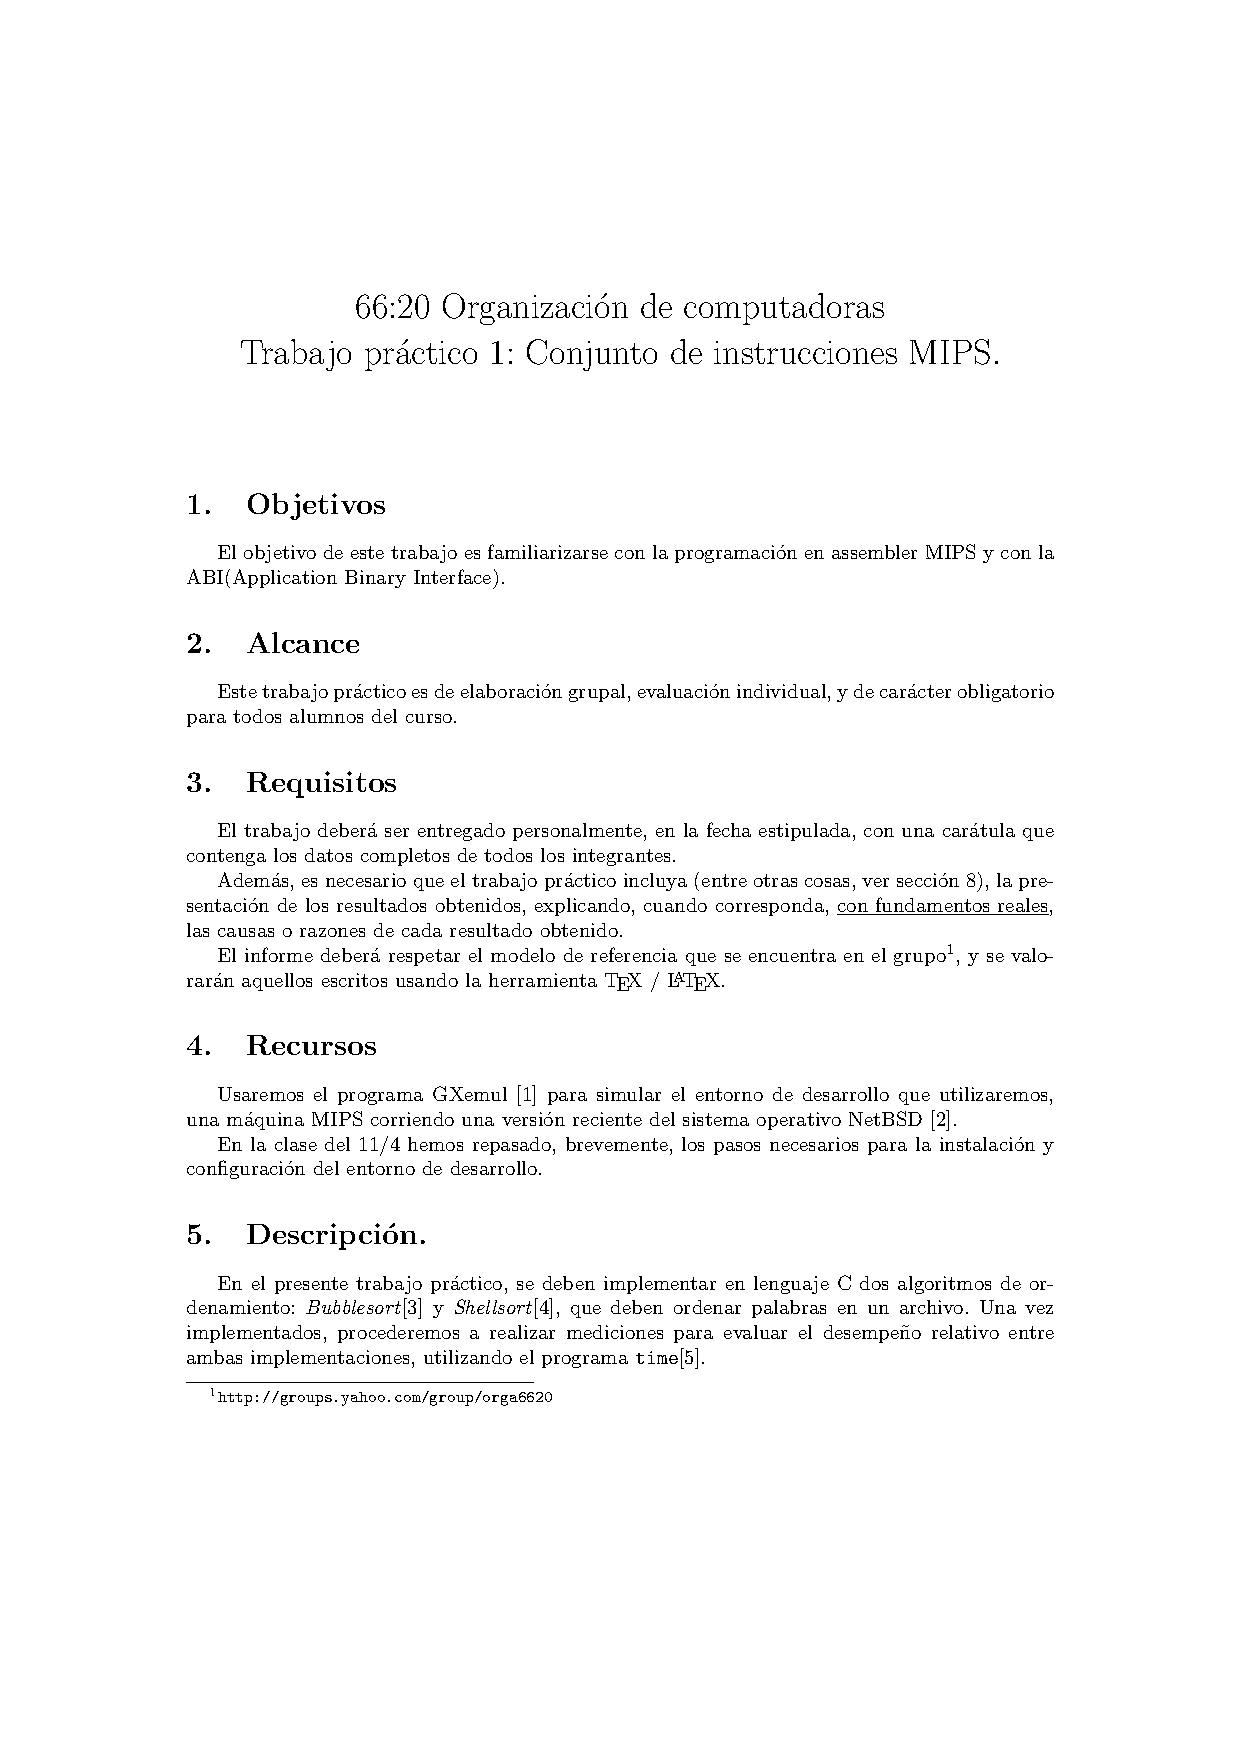
\includepdf[pages={-}]{docs/enunciado.pdf}

\clearpage
\section{Codigo fuente}\label{sec:source}
\clearpage
\definecolor{gray}{rgb}{0.5,0.5,0.5}
\lstset{
  title=\lstname,
  basicstyle=\footnotesize,
  showspaces=false,
  showstringspaces=false,
  breaklines=true,
  commentstyle=\color{gray},
  numbers=left,
  numberstyle=\tiny\color{gray},
  numbersep=5pt,
  frame=single
}

%\lstinputlisting{source/shellsort.h}
%\lstinputlisting{source/shellsort.S}

\end{document}
